\section{Selected Architectural Styles and Patterns}
This section presents the decisions about architectural styles and patterns exploited in CLup. In particular the system adopts a Client-Server architecture (see 2.6.1) and a MVC pattern (see 2.6.2).

\subsection{Client-Server Architecture}
The software to be is designed as a Client-Server system with a three-tier architecture: Presentation Level, Business Logic or Application Layer and Data Access Layer. This design architecture has already been described in section 2.1, and in it is briefly reported here only for completeness purposes.

\subsection{Model-View-Controller} 
The Model-View-Controller pattern has been selected in order to guarantee the maintainability and the reusability of the code. This software pattern, which divides the software in three parts, as can be easily deduced by his name, is particularly suitable for the development of the CLup application because it avoid a dangerous level of coupling between the different parts of the system. In particular the aim is to split the internal representation of the informations from the ways A brief description of the three parts is the following: 
\begin{itemize}
	\item \textbf{Model}: it is composed by the database and it receives user input through the Controller. 
	\item \textbf{View}: it is composed by the MobileApplication UI and the WebApplication UI and so it represents the Presentation level.
	\item \textbf{Controller}: it is composed by all the server components and it represents the logic of the system.\\
\begin{figure}[H]
\centerline{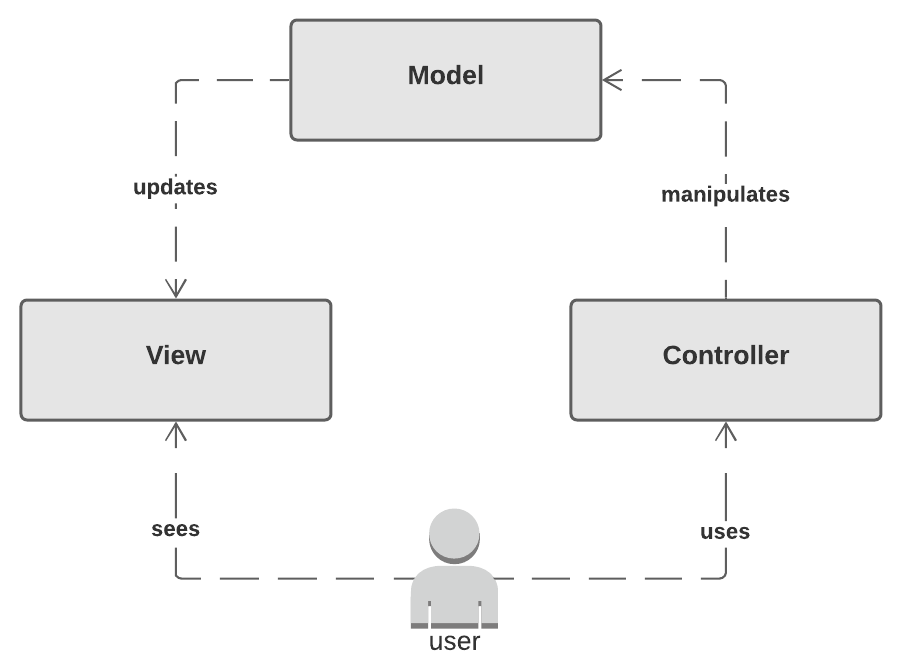
\includegraphics[scale=0.67]{./ModelViewController}}
\caption{Model-View-Controller pattern}
\end{figure}
\end{itemize}
Thanks to this it is possible to create components independently of each other and simultaneous development is simplified.   \\
Moreover the MVC schema fits particularly well with other two design patterns:
\begin{itemize}
	\item Observer pattern: lets one or more objects be notified of state changes in other objects within the system. It is fundamental in the interaction between View and Model.
	\item Factory pattern: exposes a method for creating objects, for instance both the BookingRequests and the LineUpRequests, allowing subclasses to control the actual creation process.
\end{itemize}





 
 